\chapter{ピクセル検出器}

\section{シリコン検出器}
\subsection{半導体\cite{2-1}}
固体は、絶縁体、半導体、導体の3つに大別できる。物質の電気伝導度に関して、絶縁体は非常に低い値、導体は高い値を持つ。
半導体の電気伝導度はこれらの中間であり、温度、光、磁界および微量の不純物に対し非常に敏感である。この特徴のために半導体はエレクトロニクスにおける最も重要な材料の1つになっている。
半導体は元素半導体と化合物半導体に分けられ、多くの物質がその候補となる。
元素半導体の中で代表的なものとして$\rm{Si}$があげられ、ATLASピクセル検出器に使われる半導体は$\rm{Si}$がベースとなっている。
不純物が入っていない、全ての原子が$\rm{Si}$の半導体を真性半導体と呼ぶ。真性半導体中の$\rm{Si}$は4つの$\rm{Si}$と共有結合を構成し、結晶を作る。(図\ref{pure_silicon})

\begin{figure}[bpt]\centering
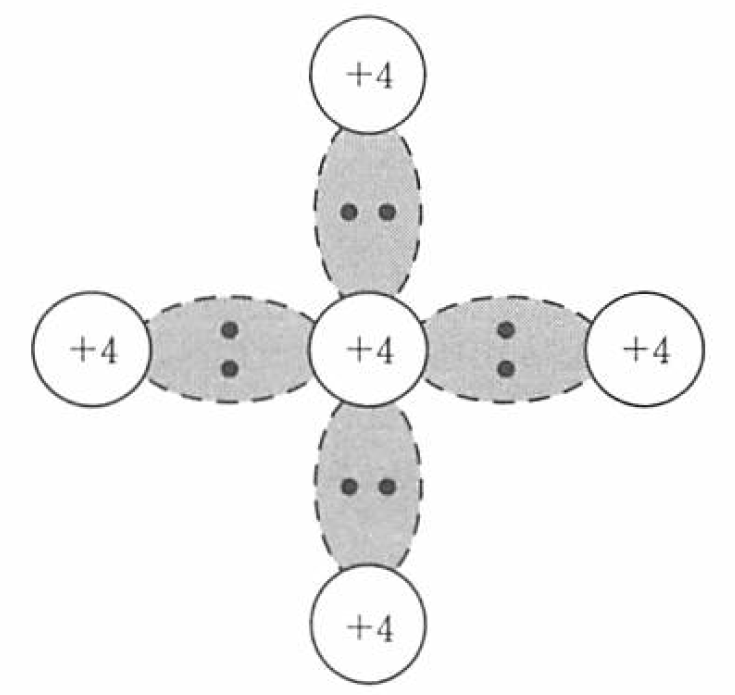
\includegraphics[width=8cm]{pure_silicon}
\caption[真性半導体中のシリコン]{真性半導体中のシリコン\cite{2-1}}
\label{pure_silicon}
\end{figure}

真性半導体に対し、$\rm{As}$などの最外殻電子を5つもつ原子を不純物としてドープしたものを$\rm{n}$型半導体、$\rm{B}$などの3つのものをドープしたものを$\rm{p}$型半導体と呼ぶ。
それぞれキャリアとして電子、ホールを持つことになり、キャリア移動の特性を組み合わせて様々なデバイスに応用することができる。

\subsection{pn接合}
$\rm{n}$型半導体と$\rm{p}$型半導体を接合し、その接合部を$\rm{pn}$接合と呼ぶ。この接合は各種半導体素子で様々な形で応用されており、ピクセル検出器にも用いられている。

$\rm{pn}$接合の最も重要な特徴は特定の方向にだけ電流が流れやすい整流性である。図\ref{pn_iv}に示すように正電圧をかけると電流は急速に増加する。
逆方向にかけた場合、始めのうちは電流はほとんど流れない。ある臨界電圧に達すると電流は急激に増大する。

\begin{figure}[bpt]\centering
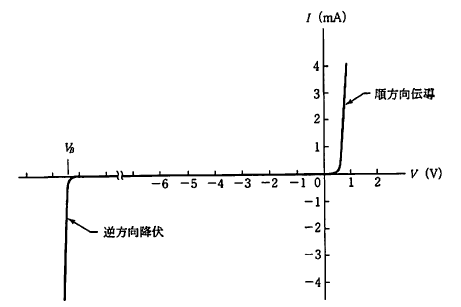
\includegraphics[width=10cm]{pn_iv}
\caption[$\rm{pn}$接合の電流$-$電圧特性]{$\rm{pn}$接合の電流$-$電圧特性\cite{2-1}}
\label{pure_silicon}
\end{figure}

逆方向電圧をかけた場合、図\ref{depletion_field}に示すように$\rm{pn}$接合付近はキャリアが存在しない空乏層領域が形成される。
この時、それぞれの半導体のエネルギー準位に差が生じている状態となっている。
印加電圧$V$と空乏層幅$W$は以下のような関係がある。
\bbb
W \propto \sqrt{V}
\eee

\begin{figure}[bpt]\centering
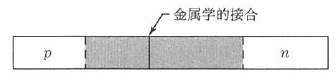
\includegraphics[width=10cm]{depletion_field}
\caption[空乏層]{空乏層\cite{2-1}}
\label{depletion_field}
\end{figure}

\subsection{検出原理}
荷電粒子が物質中を通過するとき、以下のBethe$-$Blochの公式によってエネルギーを損失する\cite{2-3}。
\bbb
-\left<\frac{\rm{d}E}{\rm{d}x}\right> &=& Kz^2\frac{Z}{A}\frac{1}{\beta^2}\left(\frac{1}{2}\rm{ln}\frac{2m_ec^2\beta^2\gamma^2T_{max}}{I^2}-\beta^2+\cdots\right)\\
\frac{\rm{d}E}{\rm{d}x}&:& 荷電粒子のエネルギー損失量[\rm{eV\cdot g^{-1}\cdot cm^2}] \\\nonumber
K&:& 4\pi N_Ar_e^2m_ec^2 = 0.307075 [\rm{MeVcm^2}] \\\nonumber
z&:& 荷電粒子の電荷量                          \\\nonumber   
Z&:& 物質の原子番号(\rm{Si} 14)                 \\\nonumber
A&:& 物質の原子量(\rm{Si} 28)\\\nonumber
m_ec^2&:& 電子の静止エネルギー(\rm{0.511MeV}) \\\nonumber
\beta&:& 光速を1とした入射粒子の速度 \\\nonumber
\gamma&:&ローレンツ因子 1/\sqrt{1-\beta^2} \\\nonumber
I&:& 励起エネルギーの期待値(シリコン 137\rm{eV}) \\\nonumber
\eee
また$T_max$は質量$M$の入射粒子による1つの電子への最大運動エネルギー移行であり、以下の式で書ける。
\bbb
T_{{\rm max}} = \frac{2m_ec^2\beta^2\gamma^2}{1+2\gamma m_e/M+\left(m_e/M\right)^2}
\eee

荷電粒子が半導体を通過したとき、そのエネルギー損失量に応じて電子・ホール対が生成し、その量を測定することができる。

\section{新型ピクセルモジュール}

新型ピクセルモジュールの構成と、各部品についての説明を以下で述べる。
\subsection{モジュールの構成}
モジュールの構成を図\ref{module_configuration}に示す。
また、モジュールの信号伝達の様子を模式的に表したものを図\ref{module_electric_overview}に示す。

\begin{figure}[bpt]\centering
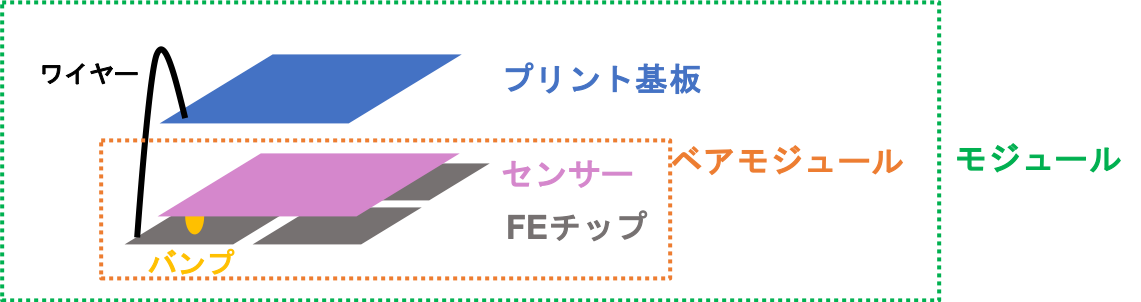
\includegraphics[width=10cm]{module_configuration}
\caption[ピクセルモジュールの構成]{ピクセルモジュールの構成}
\label{module_configuration}
\end{figure}

\begin{figure}[bpt]\centering
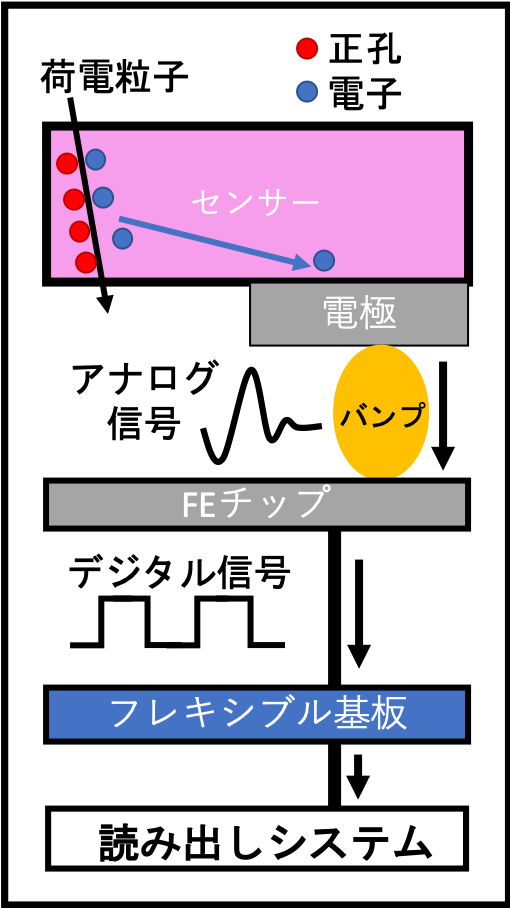
\includegraphics[width=10cm]{module_electric_overview}
\caption[信号伝達]{信号伝達}
\label{module_electric_overview}
\end{figure}

\subsubsection{モジュールの種類}
Quad, tripletなど

\subsubsection{シリコンセンサー}

\subsubsection{読み出しFEチップ}

\begin{figure}[bpt]\centering
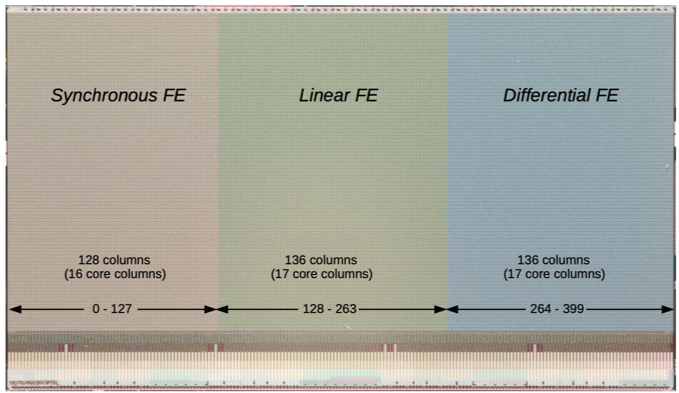
\includegraphics[width=10cm]{fechip_rd53a}
\caption[RD53A]{RD53A\cite{2-1}}
\label{fechip_rd53a}
\end{figure}

\begin{figure}[bpt]
  \begin{center}
  \begin{minipage}{0.33\hsize}
    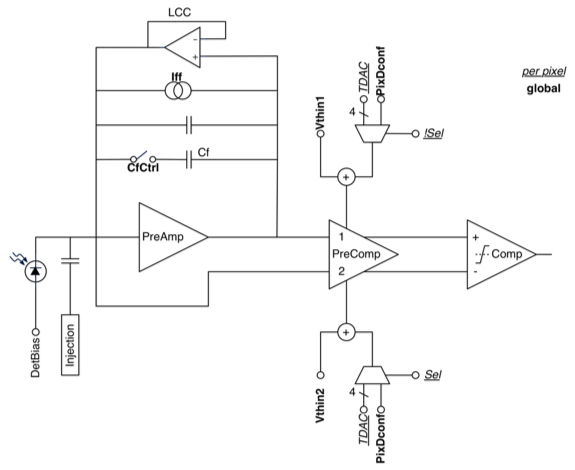
\includegraphics[width=6cm]{diff_fe}
  \end{minipage}
  \begin{minipage}{0.33\hsize}
    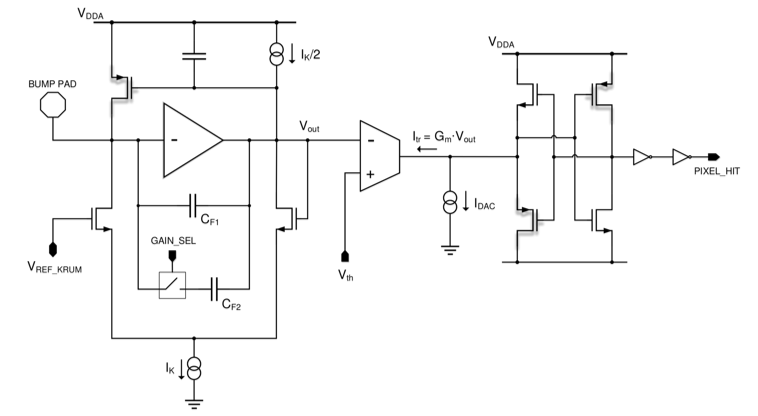
\includegraphics[width=6cm]{lin_fe}
  \end{minipage}
  \begin{minipage}{0.33\hsize}
    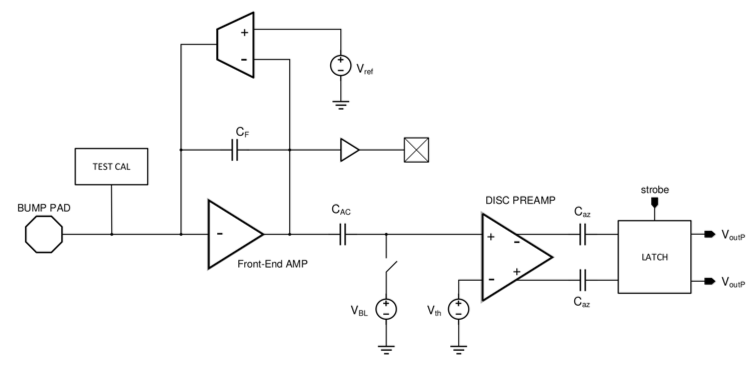
\includegraphics[width=6cm]{syn_fe}
  \end{minipage}
  \caption[アナログフロントエンド]{アナログフロントエンド\cite{2-1}}
  \label{analog_fe}
  \end{center}
\end{figure}

\begin{figure}[bpt]\centering
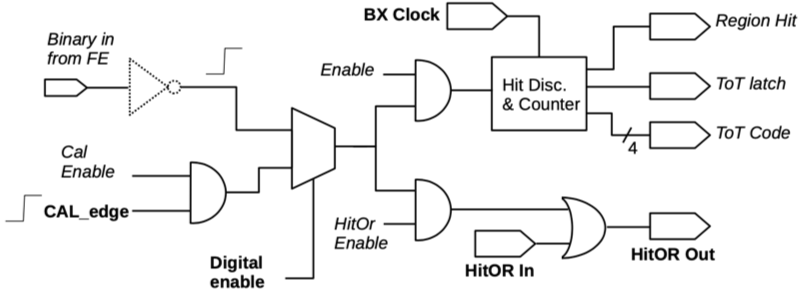
\includegraphics[width=10cm]{digital_fe}
\caption[デジタルフロントエンド]{デジタルフロントエンド\cite{2-1}}
\label{digital_fe}
\end{figure}

\subsubsection{プリント基板}

\begin{figure}[bpt]\centering
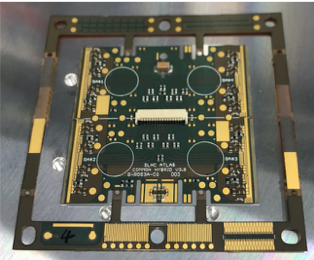
\includegraphics[width=10cm]{pcb}
\caption[プリント基板]{プリント基板}
\label{pcb}
\end{figure}

\subsubsection{モジュールキャリア}


